\documentclass[tikz,border=10pt]{standalone}
\usepackage{pgfplots}
\pgfplotsset{compat=1.18}
\usepackage{amsmath}
\usepackage{amssymb}
\definecolor{mantis}{RGB}{0, 105, 62}
\begin{document}
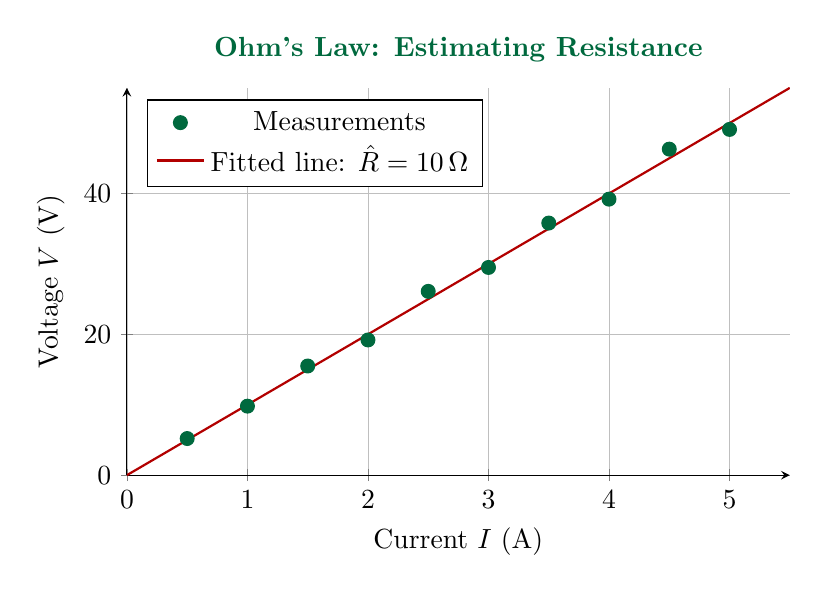
\begin{tikzpicture}
\begin{axis}[
    width=10cm,
    height=6.5cm,
    xlabel={Current $I$ (A)},
    ylabel={Voltage $V$ (V)},
    xmin=0, xmax=5.5,
    ymin=0, ymax=55,
    grid=both,
    grid style={line width=.1pt, draw=gray!30},
    major grid style={line width=.2pt,draw=gray!50},
    axis lines=left,
    legend pos=north west,
    title={\textbf{Ohm's Law: Estimating Resistance}},
    title style={font=\bfseries\color{mantis}},
]
\addplot[only marks, mark=*, mark size=2.5pt, color=mantis] coordinates {
    (0.5, 5.2) (1.0, 9.8) (1.5, 15.5) (2.0, 19.2) (2.5, 26.1)
    (3.0, 29.5) (3.5, 35.8) (4.0, 39.2) (4.5, 46.3) (5.0, 49.1)
};
\addplot[domain=0:5.5, samples=2, color=red!70!black, thick] {10*x};
\legend{Measurements, Fitted line: $\hat{R} = 10\,\Omega$}
\end{axis}
\end{tikzpicture}
\end{document}
